\documentclass[9pt, handout]{beamer}

%!TEX root = ../notas_de_clase.tex

%preamble

%language
\usepackage[spanish,es-nodecimaldot]{babel}
\usepackage[utf8]{inputenc}
\usepackage{apacite}
\usepackage[absolute,overlay]{textpos}

%packages
\usepackage[Algoritmo]{algorithm}
\usepackage{algorithmicx}
\usepackage[noend]{algpseudocode}
\usepackage{mathtools}
\setlength {\marginparwidth}{2cm}
\usepackage{todonotes}
\usepackage{amsbsy}
\usepackage{amssymb}
\usepackage{amsmath,bm}
\usepackage{dsfont}

\usepackage{xcolor}
\providecommand{\sred}[1]{\textcolor{red}{#1}}
\providecommand{\sblue}[1]{\textcolor{blue}{#1}}
\providecommand{\red}[1]{\textcolor{red}{\text{#1}}}
\providecommand{\blue}[1]{\textcolor{blue}{\text{#1}}}
\providecommand{\redb}[1]{\textcolor{red}{\textbf{#1}}}
\providecommand{\blueb}[1]{\textcolor{blue}{\textbf{#1}}}
\usepackage{graphicx}
\usepackage{fancybox}
\usepackage{booktabs}
\usepackage{caption}
\usepackage{float}
%\usepackage[longend,ruled,algochapter,linesnumbered,lined,boxed,commentsnumbered,spanish]{algorithm2e}
%\usepackage[algo2e]{algorithm2e}
\usepackage{amssymb}
\usepackage{amstext}
\usepackage{bm}
\usepackage{wrapfig}
\usepackage{subcaption} % para_unsupervised_chapter

%formatting

\usepackage[export]{adjustbox}

%caption para figuras
\captionsetup[figure]{width=.8\linewidth, font=small,labelfont={bf},name={Fig.},labelsep=period}
\captionsetup[table]{width=.8\linewidth,font=small,labelfont={bf},name={Tabla},labelsep=period}



\ifx\byn\undefined
    \definecolor{my_blue}{HTML}{C2D5FF}
    \definecolor{my_red}{HTML}{FFC2C2}
    \definecolor{my_yellow}{HTML}{FFFFE0}
\else
    \definecolor{my_blue}{HTML}{FFFFFF}
    \definecolor{my_red}{HTML}{FFFFFF}
    \definecolor{my_yellow}{HTML}{FFFFFF}
\fi


\usepackage[framemethod=TikZ]{mdframed}
\mdfdefinestyle{discusion}{%
    %linecolor=black,
    %outerlinewidth=0pt,
    roundcorner=0pt,
    innertopmargin=5pt,
    innerbottommargin=5pt,
    innerrightmargin=20pt,
    innerleftmargin=20pt,
    backgroundcolor=my_blue}

\colorlet{Green}{green!90}


\mdfdefinestyle{ejemplo}{%
    %linecolor=black,
    %outerlinewidth=0pt,
    roundcorner=0pt,
    innertopmargin=5pt,
    innerbottommargin=5pt,
    innerrightmargin=20pt,
    innerleftmargin=20pt,
    backgroundcolor=my_yellow}


\mdfdefinestyle{pendiente}{%
    style = discusion, 
    backgroundcolor=my_red}


\RequirePackage{url}



%definitions
\def\td{{\text d}}
\def\cN{{\mathcal N}}
\def\cX{{\mathcal X}} 
\def\cC{{\mathcal C}} 
\def\N{{\mathbb N}}
\def\d{{\text d}}
\def\datos{{\mathcal D}}
\def\eye{{\mathbb I}}
\def\ssum{{\scriptstyle\sum}}
\def\bepsilon{{\bm \epsilon}}
\def\tx{\tilde{x}}
\def\tX{\tilde{X}}
\def\thetaMAP{\theta_\text{MAP}}
\newcommand{\gp}{\ensuremath{\mathcal{GP}}}
\newcommand{\pr}{\ensuremath{\mathbb{P}}}
\newcommand{\x}{\ensuremath{\mathbf{x}}}
\newcommand{\z}{\ensuremath{\mathbf{z}}}
\newcommand{\cvector}{\ensuremath{\mathbf{c}}}
\newcommand{\e}{\ensuremath{\mathbf{e}}}
\newcommand{\y}{\ensuremath{\mathbf{y}}}
\newcommand{\bx}{\ensuremath{\textcolor{blue}{X}}}
\newcommand{\by}{\ensuremath{\textcolor{blue}{Y}}}
\newcommand{\rx}{\ensuremath{\textcolor{red}{X_*}}}

\newcommand{\R}{\mathbb{R}}
\newcommand{\norm}[1]{\left\lVert#1\right\rVert}




\DeclareMathOperator*{\argmax}{arg\,max}
\DeclareMathOperator*{\argmin}{arg\,min}
\DeclareMathOperator{\E}{\mathbb{E}}
\DeclareMathOperator{\V}{\mathbb{V}}
\DeclareMathOperator{\KL}{\text{KL}}
\DeclareMathOperator{\MVN}{\text{MVN}}
\newcommand\deq{\stackrel{\mathclap{\normalfont\mbox{\tiny def}}}{=}}
%\newcommand{\E}[1]{\mathbb E \left[#1\right]}
\newcommand{\trace}[1]{\text{Tr} \left[#1\right]}


\usepackage{amsthm}

%-------------------------------------------
% Newtheorem
%-------------------------------------------
\newtheorem{axioma}{\textcolor{red}{Axioma}}
\newtheorem{definicion}{Definición}
\newtheorem*{notacion}{Notación}
\newtheorem{teorema}{Teorema}
\newtheorem{corolario}{Corolario}
\newtheorem{lema}{Lema}
\newtheorem{lemaZ}{\textcolor{red}{Lema}}
\newtheorem{propiedad}{Propiedad:}
\newtheorem{proposicion}{Proposición:}
\newtheorem*{observacion}{Observación}
\newtheorem*{comentario}{Comentario}
\newtheorem*{ejemplo}{Ejemplo}
\newtheorem*{resultado}{Resultado}
\newtheorem*{propuesto}{Ejercicio propuesto}
\newtheorem*{demostracion}{Demostración} % No se usa, usar \begin{proof}\end{proof} que son por default.

%listing paackage para código
\usepackage{listings}
\usepackage{xcolor}
 
\definecolor{codegreen}{rgb}{0,0.6,0}
\definecolor{codegray}{rgb}{0.5,0.5,0.5}
\definecolor{codepurple}{rgb}{0.58,0,0.82}
\definecolor{backcolour}{rgb}{0.95,0.95,0.92}
 
\lstdefinestyle{mystyle}{
    xleftmargin=0.15\textwidth,
    linewidth=0.8\textwidth,
    backgroundcolor=\color{backcolour},   
    commentstyle=\color{codegreen},
    keywordstyle=\color{magenta},
    numberstyle=\tiny\color{codegray},
    stringstyle=\color{codepurple},
    basicstyle=\ttfamily\footnotesize,
    breakatwhitespace=true,         
    breaklines=true,                 
    captionpos=b,                    
    keepspaces=true,                 
    numbers=left,                    
    numbersep=5pt,                  
    showspaces=false,                
    showstringspaces=false,
    showtabs=false,                  
    tabsize=2
}
 
\lstset{style=mystyle}

\numberwithin{equation}{section}

\usetheme{simple}
 
\title{Clase 7: Predicciones y regresión no lineal}
\subtitle{MA5204 Aprendizaje de Máquinas}
\date{\today}
\author{Felipe Tobar} 
\titlegraphic{
\begin{figure}[htp] 
    \centering
        
\includegraphics[width=0.15\textwidth]{../img/Uchile.pdf}% 
\end{figure}
}
\institute{Department of Mathematical Engineering \&\\ Center for Mathematical Modelling\\Universidad de Chile}

\begin{document}
\begin{frame}
  \titlepage
\end{frame}

%Predicciones.
\begin{frame}{Predicciones}
	En las clases anteriores se estudió como estimar los parámetros de un modelo. Ahora se verá cómo utilizar estas estimaciones para hacer predicciones. Para esto:
	
	\begin{itemize}
		\item Se considerará un modelo $p(y|x)$, con parámetro $\theta$, del cual se han obtenido datos denotados mediante $\datos = \{(x_i,y_i)\}_{i=1}^N$.\pause
		\item Se considerará un modelo de \textbf{variable latente}: las observaciones consisten en una variable interna no observable que es perturbada por algún ruido. \\
		Por ejemplo, en el modelo lineal y gaussiano, las observaciones son de la forma:

			\begin{equation*}
				y= \underbrace{\theta^\top x}_{\text{variable latente}} + \underbrace{\epsilon}_{\text{perturbación}}
			\end{equation*}\pause
		\item De esta forma, al momento de hacer predicción, el objetivo será calcular la variable latente y no la observación (imposible de calcular). Pues esta variable latente es la esperanza de la observación.
	\end{itemize}
	
\end{frame}

%Predicciones.
\begin{frame}{Predicción \emph{plug in}}

Se denotará mediante $\hat f_\star$ e $\hat y_\star$ las predicciones de la variable latente $f$ y la observación $y$ para una nueva entrada $x_\star$, condicional a los datos observados $\datos$.\\~\ \pause

Para un modelo lineal gaussiano con estimador puntual $\hat{\theta}$, el modelo corresponde a $y=\hat{\theta}^\top x + \epsilon$. \pause Se tiene que:

\begin{itemize}
	\item Predicción de la variable latente: $\hat f_\star=\hat{\theta}^\top x_\star$ (determinista).\pause
	\item Predicción de la observación: $y=\hat{\theta}^\top x_\star + \epsilon$ (aleatoria).\pause
\end{itemize}
\vspace{1em}
Además, la aleatoriedad de $\epsilon$ permite representar esta predicción en términos de su esperanza y \emph{barras de error}. Para el caso de $\epsilon$ gaussiano son explícitas, donde con un 95\% de probabilidad, $\hat y_\star\in[\theta_{\text{MV}}^\top \tilde{x}_\star - 2\sigma,\theta_{\text{MV}}^\top \tilde{x}_\star + 2\sigma]$.
	
\end{frame}


%Predicciones.
\begin{frame}{Predicción bayesiana}

Por otro lado, cuando el parámetro $\theta$ es estimado de forma bayesiana, la posterior de $\theta$ es una distribución por lo que el modelo en sí es aleatorio. \pause De esta forma, se identifican dos fuentes de incertidumbre:

\begin{itemize}
	\item Epistemológica: dada por la distribución posterior de $\theta$.\pause
	\item Aleatoria: dada por la distribución de $\epsilon$.\pause
\end{itemize}
\vspace{1em}
Por lo tanto, para obtener una estimación de la variable latente, se debe integrar sobre las fuentes de incertidumbre (\emph{integrate-out}):

\begin{align*}
	\hat f_\star &\sim p(f_\star|x_\star,\datos) \\
	&= \int p(f_\star, \theta|x_\star,\datos)\d\theta \\
	&= \int p(f_\star|x_\star, \datos, \theta)p( \theta|\datos,x_\star)\d\theta \\
	&= \int p(f_\star|x_\star, \theta)p( \theta|\datos)\d\theta\\
	&= \E_{p( \theta|\datos)}{[p(f_\star|x_\star, \theta)]}.
\end{align*}
	
\end{frame}


%Predicciones.
\begin{frame}{Predicción bayesiana}

Si bien el cálculo de la integral anterior puede ser complejo, se tienen dos casos particulares:

\begin{itemize}
	\item \textbf{Caso gaussiano:} $p(f_\star|x_\star, \theta)p( \theta|\datos)$ corresponde al producto de dos gaussianas por lo que, de acuerdo al teorema de convolución, su integral es nuevamente una gaussiana.\pause
	\item \textbf{Caso lineal:} basta notar que $f = \theta^\top \tilde{x}_\star$ y que $\theta \sim \cN(\theta_N,\sigma^2\Lambda_n^{-1})$. De esta forma, por linealidad:
\begin{equation*}
	\hat f_\star \sim p(f_\star|x_\star,\datos) = \cN(\theta_N^\top \tilde{x}_\star,\tilde{x}_\star^\top\sigma^2\Lambda_n^{-1} \tilde{x}_\star).
\end{equation*}\pause

Además, para determinar la predicción de la observación ruidosa $y=f+\epsilon$, solo se debe incorporar el estadístico del ruido:
\begin{equation*}
	\hat y_\star\sim\cN(\theta_N^\top \tilde{x}_\star,\tilde{x}_\star^\top\sigma^2\Lambda_n^{-1} \tilde{x}_\star + \sigma^2).
\end{equation*}

\end{itemize}

\pause

Por último, a partir de la predicción bayesiana es posible obtener una predicción puntual dada por la media, donde para el caso lineal se tiene que:
\begin{equation*}
	\E[f_\star|x_\star,\datos] = \E[\theta|\datos]^\top  \tilde{x}_\star = \bar \theta^\top  \tilde{x}_\star
\end{equation*}
donde $\bar \theta$ corresponde a la media posterior de $\theta$.
	
\end{frame}

%Predicciones.
\begin{frame}{4 predicciones}

\begin{figure}[H]
	\centering
	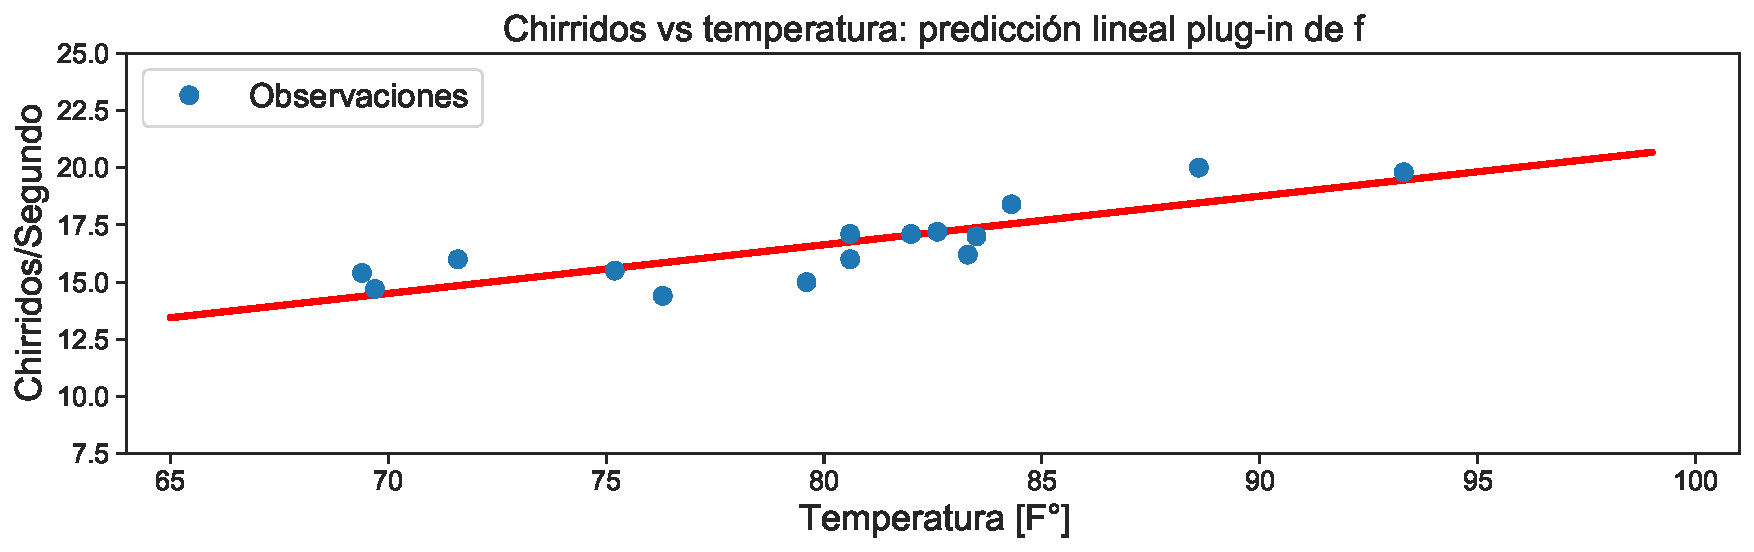
\includegraphics[width=0.57\textwidth]{../img/cap2_chirridos_pred1}
	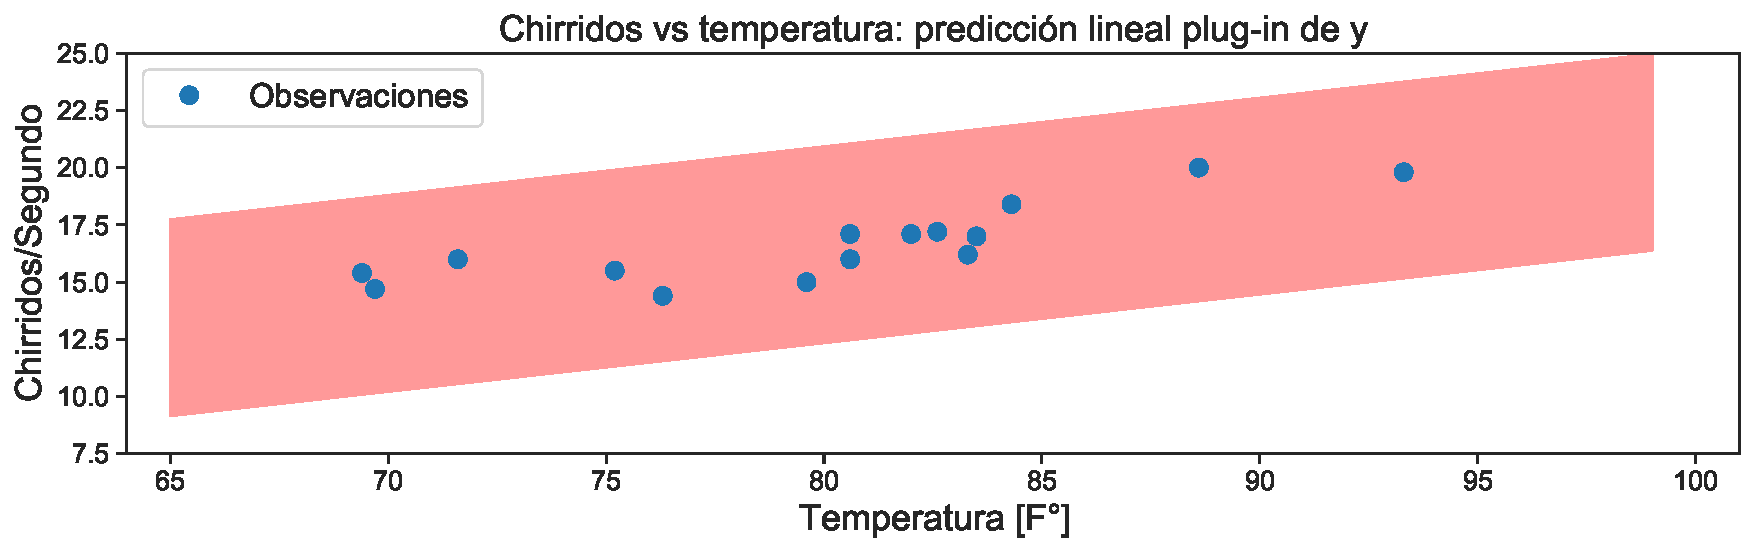
\includegraphics[width=0.57\textwidth]{../img/cap2_chirridos_pred2}
	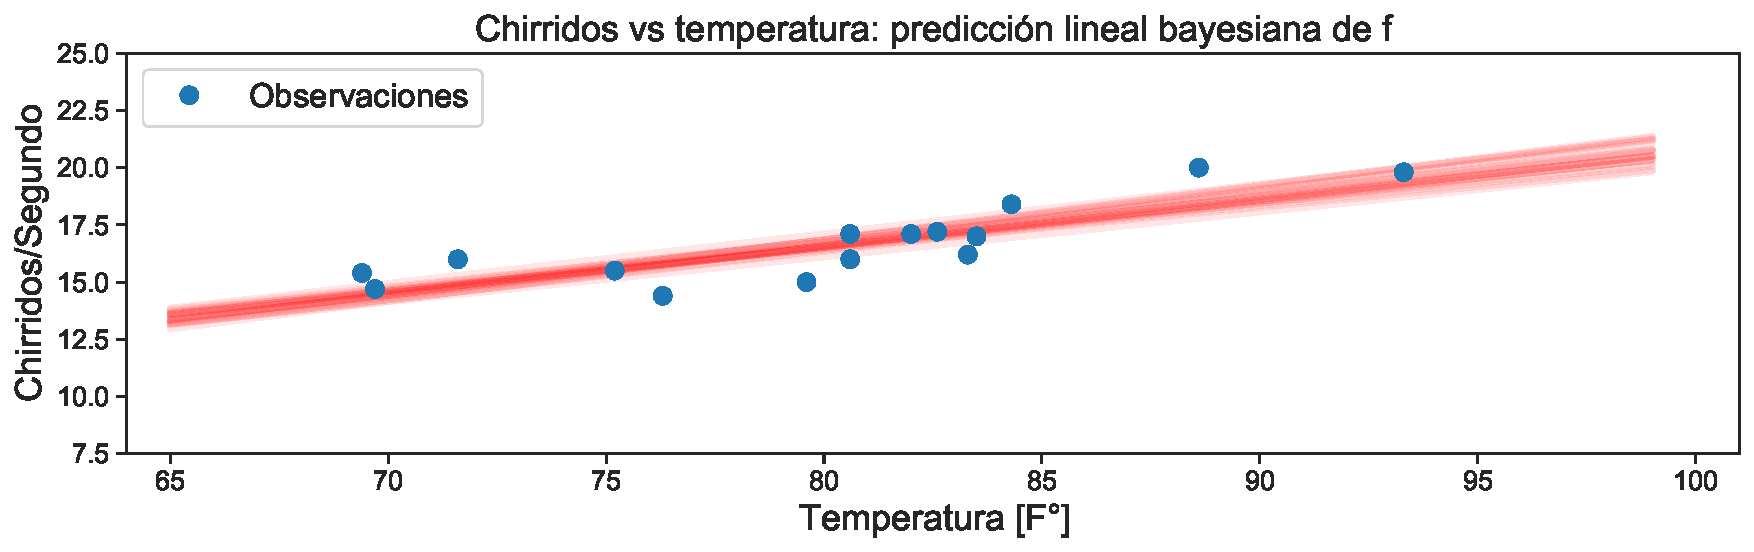
\includegraphics[width=0.57\textwidth]{../img/cap2_chirridos_pred3}
	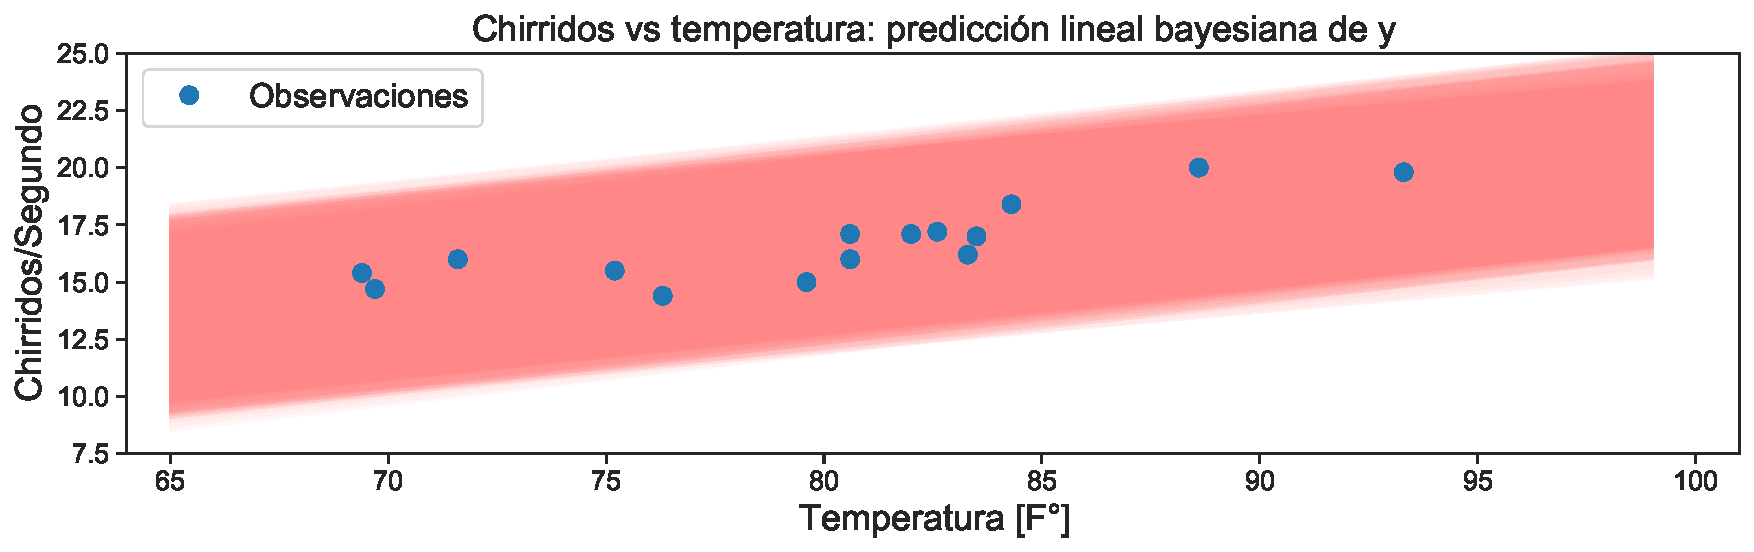
\includegraphics[width=0.57\textwidth]{../img/cap2_chirridos_pred4}
\end{figure}
	
\end{frame}

%Regresión no lineal.
\begin{frame}{Regresión no lineal}

El concepto de regresión lineal puede ser extendido mediante la aplicación de una transformación $\phi$ sobre la variable independiente $x$, construyendo un modelo lineal en la variable transformada $\phi=\phi(x)$ en lugar de en la variable original $x$. \\~\ \pause

Se considerarán transformaciones de la siguiente forma:
\begin{align*}
  \phi \colon \R^M &\to \R^D\\
  x &\mapsto \phi(x)=[\phi_1(x),\ldots,\phi_D(x)]^\top
\end{align*}
donde $\phi_i: x\in\R^M \mapsto \phi_i(x)\in\R$ son funciones escalares $\forall i=1,\ldots,D$.\\~\ \pause

De esta forma, $\phi(x_i)$ puede representar las \emph{características} de la observación cruda $x_i$.\\~\ \pause

En la práctica, la función $\phi:x\mapsto\phi(x)$ es elegida en base  al conocimiento \emph{experto} que se tenga del problema. Nos referiremos a la construcción \emph{manual} de la función $\phi$ como \emph{ingeniería de características}.
	
\end{frame}

%Modelo lineal en los parámetros.
\begin{frame}{Modelo lineal en los parámetros}

Usando la nueva variable de  características $\phi=\phi(x)$ se puede proponer un modelo lineal
\begin{equation*}
    y = \theta^\top\phi(x).
\end{equation*} \pause
Para un conjunto de observaciones $\datos = \{(x_i,y_i)\}_{i=1}^N \subset\R^M\times\R$, este modelo puede ser entrenado con un funcional de costo cuadrático:
\begin{equation*}
	J = \sum_{i=1}^N(y_i - \theta^\top\phi(x_i))^2.
	\end{equation*} \pause

Además, se puede compactar el funcional utilizando la matriz de diseño:

\begin{align*}
    \Phi = 
    \left( \begin{matrix} \phi(x_1)^\top\\
    \vdots \\
    \phi(x_N)^\top\\
    \end{matrix} \right)
     = \left( \begin{matrix} \phi_1(x_1)& \ldots & \phi_D(x_1)\\
    \vdots & \ddots & \vdots \\
    \phi_1(x_N) & \ldots & \phi_D(x_N)\\
    \end{matrix} \right)
    \qquad
    Y = \left( \begin{matrix} y_1 \\ \vdots \\ y_N \end{matrix} \right)
\end{align*}\pause
Por lo que el funcional se reescribe como $J=\norm{Y-\Phi\theta}_2^2$, cuyo mínimo es alcanzado en
\begin{align*}
    \theta{\star}&= (\Phi^\top\Phi)^{-1}\Phi^\top Y\label{eq:nolin_theta}.
\end{align*}

\end{frame}

%Modelo lineal en los parámetros.
\begin{frame}{Modelo lineal en los parámetros}

Por último, es posible realizar una regularización sobre este modelo al igual que en MCR. Por ejemplo, para la regularización de \emph{ridge}:

\begin{equation*}
    J_\rho = \norm{Y-\Phi\theta}_2^2 + \rho\left \| \theta \right \|^2,\quad \rho\in\R^+.
\end{equation*} \pause
En cuyo caso, es sabido que el funcional es minimizado en
\begin{equation*}
    \theta = (\Phi^\top\Phi+\rho\mathbb{I})^{-1}\Phi^\top Y.
\end{equation*}\pause

\textbf{Observación:} la transformación afín-lineal $\tx_i=(x_i,1)^\top$ usada al comienzo del curso, puede ser interpretada como un modelo de regresión no lineal bajo el mapa  de características

\begin{equation*}
	x\in\R^M\mapsto \phi(x)=\left(\begin{matrix}
		x\\1
	\end{matrix}\right)\in\R^{M+1}.
\end{equation*}

\end{frame}

%Ejemplos de transformaciones
\begin{frame}{Ejemplos de transformaciones}

\noindent\textbf{Función Polinomial:} $\phi=\{\phi_i\}_{i=0}^D$, donde $\phi_i(x)=x^i$, de tal forma que 
\begin{equation*}
    \Phi = \left[ \begin{matrix} 1 & x_1 & x_1^2 & \ldots & x_1^D\\
    \vdots & \vdots & \vdots & \ddots & \vdots \\
    1 & x_N & x_N^2 & \ldots & x_N^D\\
    \end{matrix} \right].
\end{equation*}\pause

\begin{itemize}
	\item De acuerdo al teorema de Stone-Weierstrass, los polinomios son densos en $\mathcal{C}([a,b])$ (funciones continuas sobre compactos), por lo que es posible aproximar cualquier función continua mediante un polinomio.\pause
	\item Una desventaja de esta  base es que puede ser inestable: para obtener una buena aproximación polinomial, generalmente se requiere un grado $D$  alto, por lo que los valores de $\phi(x)$ crecen, obviamente, de forma \emph{polinomial}.\pause
	\item Por otra parte, la interpolación polinomial sufre del fenómeno de Runge, por lo que al utilizar un grado elevado, es posible que el error de predicción en los bordes crezca indefinidamente.
\end{itemize}
	
\end{frame}


%Ejemplos de transformaciones
\begin{frame}{Ejemplos de transformaciones}

\noindent\textbf{Función Sinusoidal:} $\phi=\{\phi_i\}_{i=0}^D$, donde $\phi_i(x)=\cos\left(i\frac{2\pi}{2T}(x - b_i)\right)$, es decir:
\begin{equation*}
    \Phi = \left[ \begin{matrix}
    1 & \cos\left(1\frac{2\pi}{2T}(x_1-b_1)\right) & \ldots & \cos\left(D\frac{2\pi}{2T}(x_1-b_D)\right)\\
    \vdots & \vdots  & \ddots & \vdots \\
    1 & \cos\left(1\frac{2\pi}{2T}(x_N-b_1)\right) & \ldots & \cos\left(D\frac{2\pi}{2T}(x_N-b_D)\right)\\
    \end{matrix} \right].
\end{equation*}\pause
Una forma de evitar definir una fase, es considerar dos transformaciones por cada $\phi_i$ de la forma
\begin{equation*}
    \phi_i'(x) = \left(\sin\left(i\frac{2\pi}{2T}x\right),\ \cos\left(i\frac{2\pi}{2T}x\right)\right)
\end{equation*}\pause

\begin{itemize}
	\item Al igual que los polinomios, la base de senos y cosenos es también \emph{universal} (más aún, forman una base de Hilbert de $L^2$ en el círculo).\pause
	\item Una desventaja de la base senoidal es que solo puede replicar funciones periódicas, con un período máximo en este caso  de $T$.
\end{itemize}

\end{frame}

%Ejemplo de regresión no lineal.
\begin{frame}{Ejemplo de regresión no lineal}

Consideremos el problema de predecir la cantidad de pasajeros en una aerolínea.\\ \pause

De forma incremental, se considerarán los siguientes mapas de características:

\begin{itemize}
	\item polinomial.
	\item polinomial + senoidal (oscilatorio).
	\item polinomial + senoidal (oscilatorio) + amplitud creciente.
\end{itemize}
\pause
por lo tanto, denotando por $x$ el tiempo e $y$ la cantidad de pasajero, se considerará el siguiente modelo final:
\begin{equation*}
    y = \underbrace{\sum_{i=0}^3 \theta_i x^i}_\text{parte polinomial} + \underbrace{ \sum_{i=1}^2 \alpha_i\exp(-\tau_ix^2)\cos(\omega_i(x-\psi_i))}_\text{parte oscilatoria}.
\end{equation*} \pause
La motivación de este modelo es representar la tendencia de los datos mediante la componente polinomial y la oscilación anual mediante las componentes oscilatorias.\\

	
\end{frame}

%Ejemplo de regresión no lineal.
\begin{frame}{Ejemplo de regresión no lineal}

Se cuenta con 12 años de datos con frecuencia mensual (144 datos), de los cuales solo 9 años (108 datos) han sido usado para encontrar los parámetros del modelo y los  3 años restantes (36 datos) para validar nuestras predicciones. \pause

Los regresores obtenidos son los siguientes:


\begin{figure}[H]
    \centering
    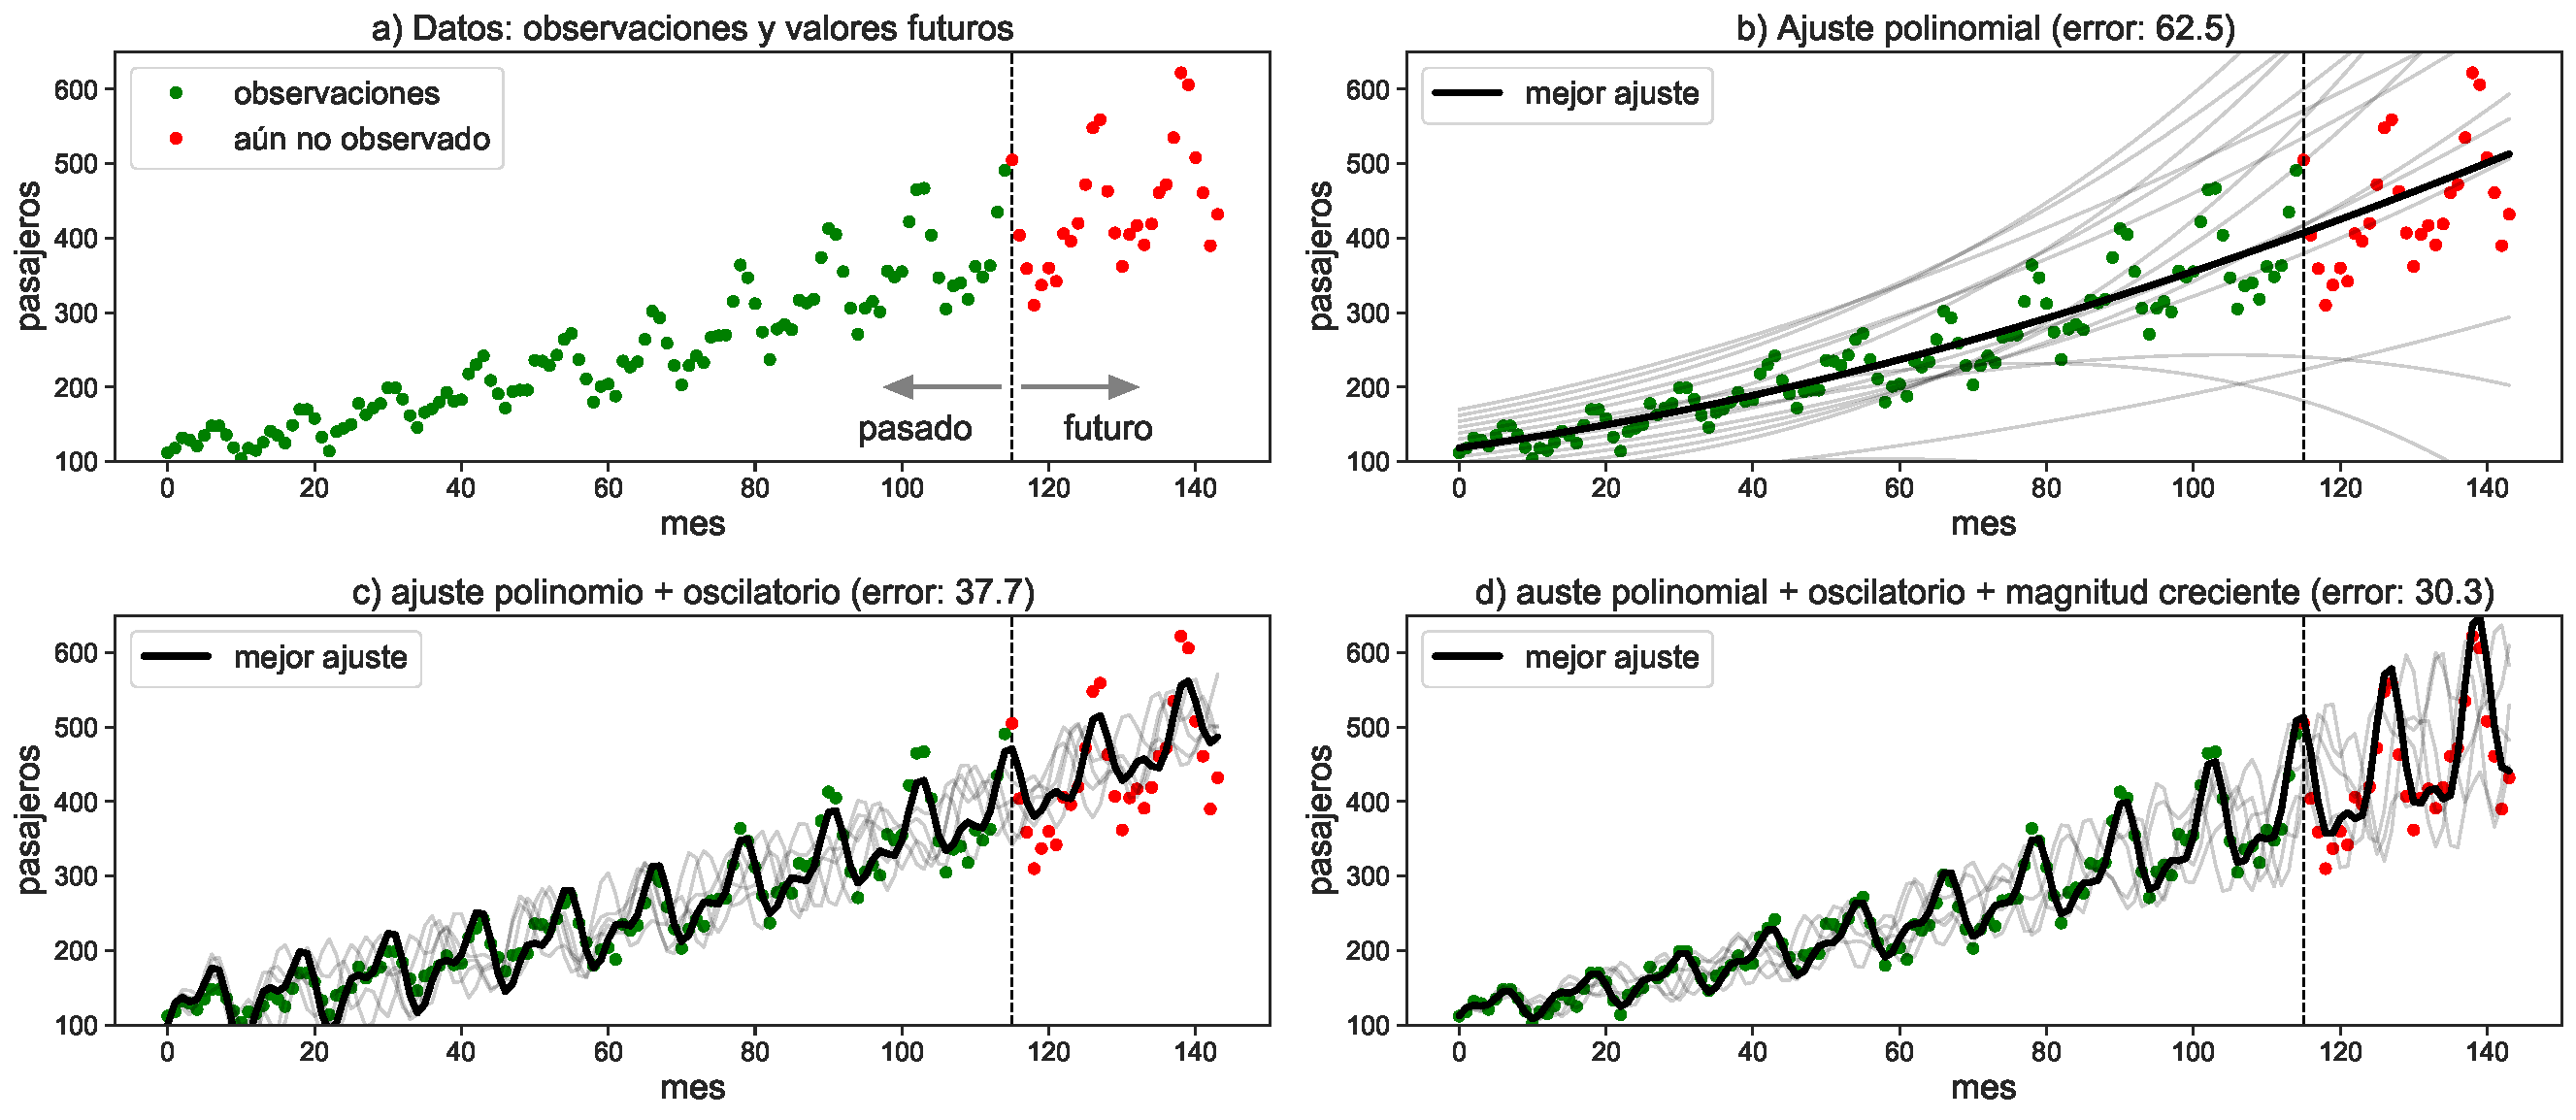
\includegraphics[width=1\textwidth, frame]{../img/cap2_pasajeros.pdf}
\end{figure}


\end{frame}

\end{document}
